\documentclass[../../main.tex]{subfiles}

\begin{document}

En este apéndice se describe todo el proceso de instalación de la aplicación bajo cualquier ordenador y sistema operativo.
Antes de entrar en los detalles es necesario remarcar, se precisa de un ordenador con unas características,a continuación se detalla una configuración mínima para que se pueda ejecutar la aplicación sin problemas:
\begin{enumerate}
\item Procesador: Intel Core i5 o AMD Ryzen 5
\item Memoria RAM: 8 GB
\item Disco SSD
\end{enumerate}

El siguiente paso es descargar el código fuente del repositorio ubicado en Github, abrimos la página del  \href{https://github.com/beaudryjp/sna_fcaR}{repositorio} y aparecerá una pantalla similar a la siguiente:

\begin{figure}[h]
\centering
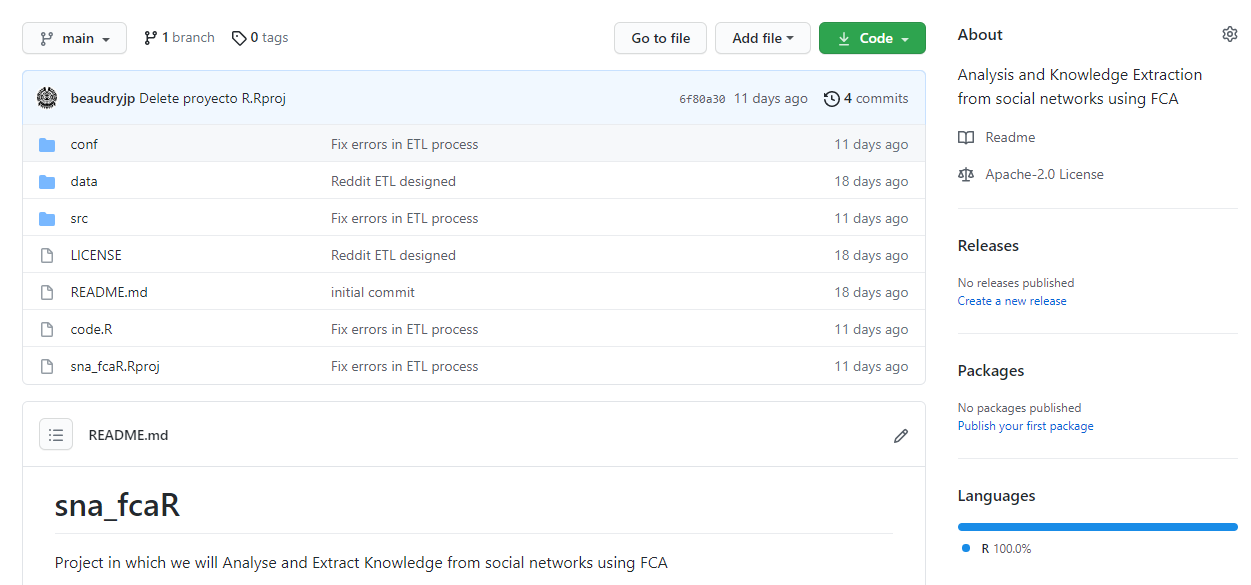
\includegraphics[width=\textwidth]{images/0_apendices/github1.png}
\caption{Repositorio del código fuente de la aplicación}
\end{figure}

En dicha pantalla hay que pulsar sobre el botón \textit{CODE} y posteriormente \textit{Download ZIP}, esto descargará un fichero comprimido con todo el código fuente del proyecto el cual puede ser abierto por las aplicaciones nativas de descompresión de ficheros de cualquier sistema operativo. \\


Para el siguiente paso es necesario disponer de un servidor de base de datos ya existente o instalar uno nuevo, para este presente trabajo se utiliza la herramienta Docker\cite{doc10}, el cual gestionará dos contenedores, una maquina virtual de con el servidor de base de datos MariaDB\cite{doc11} y una maquina virtual con el gestor de base de datos phpMyAdmin\cite{doc12} ya preconfigurada.\\

\textit{NOTA: } Si la instalación se hace bajo el sistema operativo Windows, es necesario disponer de la versión 10 del mismo y tener instalado el Subsistema de Linux para Windows.
En el siguiente \href{https://docs.microsoft.com/en-us/windows/wsl/install-win10}{enlace} viene detallado los pasos a seguir para la instalación de dicho subsistema.\\

Se recomienda instalar Docker con las opciones que aparecen por defecto, una vez instalado la aplicación Docker, es necesario abrir una ventana de terminal (En Linux/MacOS: Terminal, En Windows: PowerShell) y ejecutar los siguientes comandos en el siguiente orden:

\begin{itemize}
\item Para el contenedor MariaDB con los  parámetros:
\begin{itemize}
\item[$\ast$] \textit{-p}: El puerto interno y externo en el que correo el servicio MariaDB.
\item[$\ast$]\textit{-name}: El nombre del contenedor.
\item[$\ast$] \textit{-e}: Establecemos como variable de entorno la contraseña del usuario \textbf{root}, remarcar que es recomendable cambiar la contraseña a una más segura si se pone la aplicación en producción.
\item[$\ast$] \textit{-d}: Indicar que el contenedor funcione en segundo plano.
\end{itemize}
\end{itemize}
\begin{lstlisting}
docker run -p 3306:3306  --name mariadb -e MYSQL_ROOT_PASSWORD=root123 -d mariadb/server
\end{lstlisting}

\vskip 0.2in

\begin{itemize}
\item Para el contenedor phpMyAdmin con los parámetros:
\begin{itemize}
\item[$\ast$] \textit{-p}: El puerto interno y externo en el que correo el servicio phpMyAdmin.
\item[$\ast$]\textit{-name}: El nombre del contenedor.
\item[$\ast$] \textit{--link}: Enlazamiento de este contenedor con el contenedor del servidor de base de datos MariaDB.
\item[$\ast$] \textit{-d}: Indicar que el contenedor funcione en segundo plano.
\end{itemize}
\end{itemize}
\begin{lstlisting}
docker run --name my-own-phpmyadmin -d --link mariadb:db -p 8081:80 phpmyadmin/phpmyadmin
\end{lstlisting}

\vskip 0.2in

Una vez ejecutados estos dos comandos, tendremos dos contenedores con dos servicios diferentes en funcionamiento y en segundo plano. Para comprobar el funcionamiento de dichos contenedores se ejecuta el siguiente comando:

\begin{lstlisting}
docker ps -a
\end{lstlisting}

\vskip 0.2in

Para la creación de la base de datos hay ir a la carpeta descargada del código fuente y abrir el fichero \textit{conf/database.sql}, una vez abierto se copia todo el contenido del mismo.
Posteriormente, para acceder al gestor de base datos hay que abrir un navegador y acceder a la siguiente dirección \href{127.0.0.1:8081}{127.0.0.1:8081}, pinchar en la pestaña \textit{SQL} y pegar el contenido copiado anteriormente. \\

Por último, es necesario instalar R\cite{doc16} y RStudio Desktop\cite{doc15} en el ordenador ya que el primero es el soporte para el lenguaje en sí y el segundo es el entorno de desarrollo, así mismo se utiliza este entorno para compilar y ejecutar el código fuente para desplegar la aplicación web. \\
Una vez instalado ambos ya se puede empezar a trabajar con R y RStudio, para abrir el proyecto hay que ir a la carpeta del código fuente y abrir el fichero \textit{sna\_fcaR.Rproj}, esto abrirá proyecto en el entorno de desarrollo y desplegar la aplicación web solo hay que pinchar en el botón \textit{Run App}. \\

\end{document}